%% For double-blind review submission, w/o CCS and ACM Reference (max submission space)
\documentclass[sigconf]{acmart}
\settopmatter{printfolios=true,printccs=false,printacmref=false}
%% For double-blind review submission, w/ CCS and ACM Reference
%\documentclass[sigplan,review,anonymous]{acmart}\settopmatter{printfolios=true}
%% For single-blind review submission, w/o CCS and ACM Reference (max submission space)
%\documentclass[sigplan,review]{acmart}\settopmatter{printfolios=true,printccs=false,printacmref=false}
%% For single-blind review submission, w/ CCS and ACM Reference
%\documentclass[sigplan,review]{acmart}\settopmatter{printfolios=true}
%% For final camera-ready submission, w/ required CCS and ACM Reference
%\documentclass[sigplan]{acmart}\settopmatter{}


%% Conference information
%% Supplied to authors by publisher for camera-ready submission;
%% use defaults for review submission.
% \acmConference[PPoPP'26]{ACM SIGPLAN Annual Symposium on Principles and Practice of Parallel Programming}{January 31--February 04, 2026}{Sydney, Australia}
\acmYear{2026}
\acmISBN{} % \acmISBN{978-x-xxxx-xxxx-x/YY/MM}
\acmDOI{} % \acmDOI{10.1145/nnnnnnn.nnnnnnn}
\startPage{1}

%% Copyright information
%% Supplied to authors (based on authors' rights management selection;
%% see authors.acm.org) by publisher for camera-ready submission;
%% use 'none' for review submission.
\setcopyright{none}
%\setcopyright{acmcopyright}
%\setcopyright{acmlicensed}
%\setcopyright{rightsretained}
%\copyrightyear{2018}           %% If different from \acmYear

%% Bibliography style
\bibliographystyle{ACM-Reference-Format}
%% Citation style
%\citestyle{acmauthoryear}  %% For author/year citations
%\citestyle{acmnumeric}     %% For numeric citations
%\setcitestyle{nosort}      %% With 'acmnumeric', to disable automatic
                            %% sorting of references within a single citation;
                            %% e.g., \cite{Smith99,Carpenter05,Baker12}
                            %% rendered as [14,5,2] rather than [2,5,14].
%\setcitesyle{nocompress}   %% With 'acmnumeric', to disable automatic
                            %% compression of sequential references within a
                            %% single citation;
                            %% e.g., \cite{Baker12,Baker14,Baker16}
                            %% rendered as [2,3,4] rather than [2-4].


%%%%%%%%%%%%%%%%%%%%%%%%%%%%%%%%%%%%%%%%%%%%%%%%%%%%%%%%%%%%%%%%%%%%%%
%% Note: Authors migrating a paper from traditional SIGPLAN
%% proceedings format to PACMPL format must update the
%% '\documentclass' and topmatter commands above; see
%% 'acmart-pacmpl-template.tex'.
%%%%%%%%%%%%%%%%%%%%%%%%%%%%%%%%%%%%%%%%%%%%%%%%%%%%%%%%%%%%%%%%%%%%%%


%% Some recommended packages.
\usepackage{booktabs}   %% For formal tables:
                        %% http://ctan.org/pkg/booktabs
\usepackage{subcaption} %% For complex figures with subfigures/subcaptions
                        %% http://ctan.org/pkg/subcaption

\usepackage[ruled,linesnumbered]{algorithm2e}
\usepackage{graphicx}
\usepackage{textcomp}
\usepackage{pifont}
\usepackage{makecell}
\usepackage{url}
\usepackage{multirow}
\usepackage[switch]{lineno}
\usepackage{diagbox}
\usepackage{threeparttable}
\usepackage{bbding}
\usepackage{fancyvrb}
\usepackage{tablefootnote}
\usepackage{enumitem}
\usepackage{tabularx}
\usepackage{ulem}
\usepackage{array}
\usepackage{bigstrut}
\newcommand{\yellowcomment}[1]{\todo[inline,color=yellow!40,size=\small]{#1}}
\newcommand{\tabincell}[2]{\begin{tabular}[t]{@{}#1@{}}#2\end{tabular}}
\usepackage{listings}
\usepackage{bigstrut}
\usepackage{makecell}
\makeatletter
\theoremstyle{definition}
\newtheorem{definition}{Definition}[section]
\let\orig@lstnumber=\thelstnumber
\newcommand\lstsetnumber[1]{\gdef\thelstnumber{#1}}
\newcommand\lstresetnumber{\global\let\thelstnumber=\orig@lstnumber}

\definecolor{codegreen}{rgb}{0,0.6,0}
\definecolor{codepurple}{rgb}{0.58,0,0.82}

\definecolor{diffstart}{named}{gray}
\definecolor{diffincl}{named}{blue}
\definecolor{diffrem}{named}{orange}
\lstdefinelanguage{diff}{
  %basicstyle=\fontsize{6.5}{6}\ttfamily,
  basicstyle=\scriptsize\ttfamily,
  morecomment=[f][\color{diffstart}]{@@},
  morecomment=[f][\color{diffincl}]{+\ },
  morecomment=[f][\color{diffrem}]{-\ },
}

\lstdefinestyle{mystyle}{
	% backgroundcolor=\color{backcolour},   
	commentstyle=\color{codegreen},
	keywordstyle=\color{magenta},
	numberstyle=\tiny,
	stringstyle=\color{codepurple},
	% basicstyle=\linespread{0.7}\ttfamily\scriptsize,
	basicstyle=\fontsize{6.5}{6}\ttfamily,
	breakatwhitespace=false,         
	breaklines=true,                 
	captionpos=b,                    
	keepspaces=true,                 
	numbers=left,                    
	numbersep=5pt,                  
	showspaces=false,                
	showstringspaces=false,
	showtabs=false,                  
	tabsize=2,
	aboveskip=0pt,
	belowskip=0pt,
	xleftmargin=2em,
	xrightmargin=0em,
	frame=topline,
	mathescape=true,
	fontadjust=true
}

\lstset{style=mystyle}
% \newcommand{\yf}[1]{{\color{red} YF: #1}}

%\usepackage{minted}

%
% defining the \BibTeX command - from Oren Patashnik's original BibTeX documentation.
\def\BibTeX{{\rm B\kern-.05em{\sc i\kern-.025em b}\kern-.08emT\kern-.1667em\lower.7ex\hbox{E}\kern-.125emX}}

%\settopmatter{printfolios=true,printacmref=false} % Removes citation information below abstract
%\setcopyright{none}
%\renewcommand\footnotetextcopyrightpermission[1]{} % removes footnote with conference information in first column
% Rights management information. 
% This information is sent to you when you complete the rights form.
% These commands have SAMPLE values in them; it is your responsibility as an author to replace
% the commands and values with those provided to you when you complete the rights form.
%
% These commands are for a PROCEEDINGS abstract or paper.
%\copyrightyear{2018}
%\acmYear{2018}
%\setcopyright{acmlicensed}
% \acmConference[PPoPP'26]{ACM SIGPLAN Annual Symposium on Principles and Practice of Parallel Programming}{January 31--February 04, 2026}{Sydney, Australia}
% \acmYear{2026}
% \acmConference[]{}{}
\acmConference[ICS'2025]{The 39th ACM International Conference on
  Supercomputing}{June 9--11, 2025}{Salt Lake City, USA}
\acmISBN{} % \acmISBN{978-x-xxxx-xxxx-x/YY/MM}
\acmDOI{} % \acmDOI{10.1145/nnnnnnn.nnnnnnn}
% \startPage{1}
\settopmatter{printacmref=false}

\setcopyright{none}
%
% These commands are for a JOURNAL article.
%\setcopyright{acmcopyright}
%\acmJournal{TOG}
%\acmYear{2018}\acmVolume{37}\acmNumber{4}\acmArticle{111}\acmMonth{8}
%\acmDOI{10.1145/1122445.1122456}

%
% Submission ID. 
% Use this when submitting an article to a sponsored event. You'll receive a unique submission ID from the organizers
% of the event, and this ID should be used as the parameter to this command.
%\acmSubmissionID{123-A56-BU3}

%
% The majority of ACM publications use numbered citations and references. If you are preparing content for an event
% sponsored by ACM SIGGRAPH, you must use the "author year" style of citations and references. Uncommenting
% the next command will enable that style.
% \citestyle{acmauthoryear}
%\hypersetup{draft}
%
% end of the preamble, start of the body of the document source.

\begin{document}


%% Title information
\title[MatrixFold: Acceleration of Mixed-Precision Alphafold Inference on CPU]{MatrixFold: Hardware-Aware Acceleration of Mixed-Precision AlphaFold Inference on Manycore CPUs with Outer-Product Units}         %% [Short Title] is optional;
%% when present, will be used in
%% header instead of Full Title.
%\titlenote{For simple use only}             %% \titlenote is optional;
%% can be repeated if necessary;
%% contents suppressed with 'anonymous'
%\subtitle{Check the format}                     %% \subtitle is optional
%\subtitlenote{Everything should just work}       %% \subtitlenote is optional;
%% can be repeated if necessary;
%% contents suppressed with 'anonymous'


%% Author information
%% Contents and number of authors suppressed with 'anonymous'.
%% Each author should be introduced by \author, followed by
%% \authornote (optional), \orcid (optional), \affiliation, and
%% \email.
%% An author may have multiple affiliations and/or emails; repeat the
%% appropriate command.
%% Many elements are not rendered, but should be provided for metadata
%% extraction tools.

\author{} %% fill in for the camera-ready version with the format commented out below
%% Author with single affiliation.
% \author{First1 Last1}
% \authornote{with author1 note}          %% \authornote is optional;
%                                         %% can be repeated if necessary
% \orcid{nnnn-nnnn-nnnn-nnnn}             %% \orcid is optional
% \affiliation{
%   \position{Position1}
%   \department{Department1}              %% \department is recommended
%   \institution{Institution1}            %% \institution is required
%   \streetaddress{Street1 Address1}
%   \city{City1}
%   \state{State1}
%   \postcode{Post-Code1}
%   \country{Country1}                    %% \country is recommended
% }
% \email{first1.last1@inst1.edu}          %% \email is recommended

% %% Author with two affiliations and emails.
% \author{First2 Last2}
% \authornote{with author2 note}          %% \authornote is optional;
%                                         %% can be repeated if necessary
% \orcid{nnnn-nnnn-nnnn-nnnn}             %% \orcid is optional
% \affiliation{
%   \position{Position2a}
%   \department{Department2a}             %% \department is recommended
%   \institution{Institution2a}           %% \institution is required
%   \streetaddress{Street2a Address2a}
%   \city{City2a}
%   \state{State2a}
%   \postcode{Post-Code2a}
%   \country{Country2a}                   %% \country is recommended
% }
% \email{first2.last2@inst2a.com}         %% \email is recommended
% \affiliation{
%   \position{Position2b}
%   \department{Department2b}             %% \department is recommended
%   \institution{Institution2b}           %% \institution is required
%   \streetaddress{Street3b Address2b}
%   \city{City2b}
%   \state{State2b}
%   \postcode{Post-Code2b}
%   \country{Country2b}                   %% \country is recommended
% }
% \email{first2.last2@inst2b.org}         %% \email is recommended


%% Remove these two lines for the camera-ready version
\fancyhead{}  % clears the header fields that trigger HotCRP format checker
\renewcommand\footnotetextcopyrightpermission[1]{} % removes the ACM copyright footnote

%% Abstract
%% Note: \begin{abstract}...\end{abstract} environment must come
%% before \maketitle command
\begin{abstract}
	AlphaFold2 has achieved remarkable accuracy in protein structure prediction, yet its high computational and memory costs remain a significant barrier to large-scale deployment. While prior optimization efforts have been predominantly GPU-centric, the potential for CPU acceleration remains largely unexplored. This paper introduces MatrixFold, the first systematic study of quantized AlphaFold2 inference on a many-core CPU architecture. Targeting 72F processor with dedicated matrix units and on-package memory, we implement a series of computation and communication optimizations. These include highly optimized GEMM kernels, hardware-based communication mechanisms, and adaptive parallelism strategies to efficiently leverage the many-core resources. On CASP14 benchmarks, MatrixFold demonstrates high structural accuracy with TM-scores above 0.7. While its performance is comparable to GPU-based FastFold on short sequences, it shows a significant advantage on long sequences, achieving inference speedups of 1.2$\times$ to 3.2$\times$ over FastFold on the NVIDIA A800 GPU and 1.5$\times$ to 5.5$\times$ over Open-Omics-AlphaFold on Intel Xeon w9-3495X.
\end{abstract}
% \keywords{AlphaFold2, Protein Structure Prediction, Mixed-Precision Inference, Many-core CPU, Matrix Unit, Outer Product Unit}


%% \maketitle
%% Note: \maketitle command must come after title commands, author
%% commands, abstract environment, Computing Classification System
%% environment and commands, and keywords command.
\maketitle

\section{Introduction}

Protein structure prediction has long been recognized as one of the central challenges in computational biology, due to its critical role in understanding biological functions and developing novel therapeutics.~\cite{anfinsen1973principles} Traditional approaches, such as homology modeling and physics-based simulations, have achieved partial success but often suffer from limited accuracy or prohibitive computational cost. The release of AlphaFold2~\cite{jumper2021highly,evans2021protein} by DeepMind marked a major breakthrough in this field, delivering unprecedented accuracy in predicting three-dimensional protein structures from amino acid sequences. Its impact has extended across biology~\cite{perrakis2021ai}, protein design~\cite{goverde2023novo,wang2024protein}, and drug discovery~\cite{thornton2021alphafold,nussinov2023alphafold}, making large-scale deployment of AlphaFold2 inference increasingly desirable.
However, the adoption of AlphaFold2 in practical scenarios remains constrained by its high computational cost. A single inference typically requires substantial hardware resources, which limits its accessibility and large-scale deployment.

To address this challenge, recent efforts have focused on accelerating AlphaFold2 on GPUs. These works leverage techniques such as kernel fusion, memory optimization, and reduced-precision computation (e.g.,BF16) to improve inference efficiency. While these studies demonstrate substantial performance speedups, they are almost exclusively GPU-centric. In contrast, CPU-based acceleration of AlphaFold2 has received little attention. This lack of exploration is notable given that CPUs remain the dominant computing platform in many large-scale clusters, supercomputers, and cloud environments. Moreover, the implementations of AlphaFold2 are typically restricted to FP32 or BF16 precision, leaving aggressive quantization strategies such as FP16 and INT8 completely unexplored.

At the same time, modern CPUs are undergoing architectural evolution that brings them closer to accelerators in terms of matrix computation capability. For example, Intel has recently introduced the Advanced Matrix Extensions (AMX)~\cite{intel2022amx} in its latest processors, and Arm has developed Scalable Matrix Extensions (SME)~\cite{weidmann2021introducing} to enhance performance on modern many-core architectures. These hardware features enable CPUs to execute matrix-heavy operations with significantly higher throughput, narrowing the performance gap with GPUs for certain classes of workloads. Moreover, these matrix extensions are explicitly designed to support reduced-precision formats, making CPUs an emerging platform where quantization can play a central role in performance optimization.

The 72F processor offers a unique opportunity to revisit CPU-based acceleration of AlphaFold2. Unlike conventional CPUs, the 72F adopts a many-core architecture with eight NUMA domains. Each core is equipped with a dedicated matrix unit capable of high-throughput computation, while a high-bandwidth on-package memory sits between DDR and cache to mitigate the memory bottleneck. 
Combined with its native support for FP16 and INT8 computation, the 72F is particularly well-suited for exploring the impact of quantization on large-scale models such as AlphaFold2.

% 矩阵单元一般对与低精度计算有更好的支持。在Intel AMX中，单条BF16矩阵指令可以执行1024次运算，而INT8则可以执行2048次运算。在ARM SME中，单条INT8外积指令也可以执行FP16或BF16两倍的计算量。因此量化是提升矩阵单元利用率的关键技术。
% Model quantization has emerged as a key technique to improve the efficiency of deep learning inference by reducing both memory footprint and computational cost. By converting high-precision floating-point operations into low-precision integer arithmetic, quantization enables better utilization of hardware resources such as matrix units, while also reducing memory bandwidth pressure. Recent studies have demonstrated that INT8 quantization can achieve substantial speedups with negligible accuracy degradation for vision and language models.

% Despite its effectiveness, quantization has not been systematically applied to AlphaFold2. The model's heterogeneous computation patterns, including attention, triangular updates, and geometry-based transformations, make straightforward quantization non-trivial. Moreover, maintaining structural accuracy under low-precision computation is particularly challenging for AlphaFold2, as minor numerical errors can accumulate and lead to significant deviations in predicted atomic coordinates. These challenges highlight the need for specialized quantization strategies that are tailored to AlphaFold2's architecture and workloads, particularly in the context of CPU execution with matrix units.

% To address these challenges, we introduce MatrixFold, an efficient implementation of AlphaFold2 for inference. MatrixFold is designed to fully exploit the capabilities of modern many-core CPUs with matrix units, while incorporating INT8 quantization to maximize throughput. Our contributions are as follows:
Optimizing AlphaFold2 on the 72F CPU presents several challenges. First, the model is dominated by large-scale dense linear algebra, requiring efficient matrix multiplication kernels that can fully exploit the matrix units of each core. Second, the processor's many-core, multi-NUMA design necessitates careful handling of communication across memory domains to avoid bandwidth contention and excessive synchronization. Third, the adoption of reduced-precision inference on CPUs introduces new complexity, as FP16 and INT8 quantization must be integrated without sacrificing model accuracy. Finally, the variable length of protein sequences makes parallelization non-trivial: overly aggressive parallelism on short sequences can lead to small per-thread workloads, synchronization overheads, and costly cross-NUMA communication.

To overcome these challenges, we make several design choices. We develop a high-performance GEMM implementation tailored to the 72F's matrix units, ensuring that the dominant computation is efficiently executed. We design a shared-memory communication mechanism optimized for multi-NUMA systems, reducing inter-node data transfer costs. We enable FP16 inference and implement INT8 quantization, providing the first demonstration of quantized AlphaFold2 inference on CPUs. Furthermore, we introduce a parallelism detection mechanism that adaptively selects thread counts to balance workload granularity against synchronization and communication overhead.
In this work, we present MatrixFold, a systematic study of AlphaFold2 optimization on CPUs, targeting the 72F architecture. Our contributions are as follows:
\begin{itemize}
    \item We present a systematic study and implementation of mix-precision (FP16 and INT8) AlphaFold2 inference on a many-core CPU architecture. 
    \item We propose a suite of computation and communication optimizations specifically tailored for the target 72F processor, leveraging its dedicated matrix units and multi-NUMA architecture.
    \item We conduct a comprehensive evaluation on the CASP14 dataset, demonstrating that MatrixFold achieves a significant performance advantage on long sequences, outperforming the state-of-the-art GPU implementation, FastFold on an NVIDIA A800 GPU, by 1.2$\times$ to 3.2$\times$. 
    \item We validate that our mixed-precision  strategy achieves substantial performance gains without compromising prediction accuracy, confirming the viability and effectiveness of low-precision inference for AlphaFold2 on CPUs.
    % \item We design a set of high-performance GEMM kernels leveraging matrix units to accelerate the inference of AlphaFold2. 
    % \item We enable quantized inference on CPUs by implementing both FP16 and INT8 execution, moving beyond the conventional FP32/BF16 precision levels.
    % \item We design NUMA-aware parallelization and memory optimizations that exploit the 72F's many-core design and high-bandwidth on-package memory.
    % \item We provide a comprehensive evaluation demonstrating that our approach achieves substantial performance improvements while maintaining accuracy.
\end{itemize}
\section{Background}
\label{sec:background}

\subsection{SVE and SME Units on Arm CPUs}
\begin{figure}
    \centering
    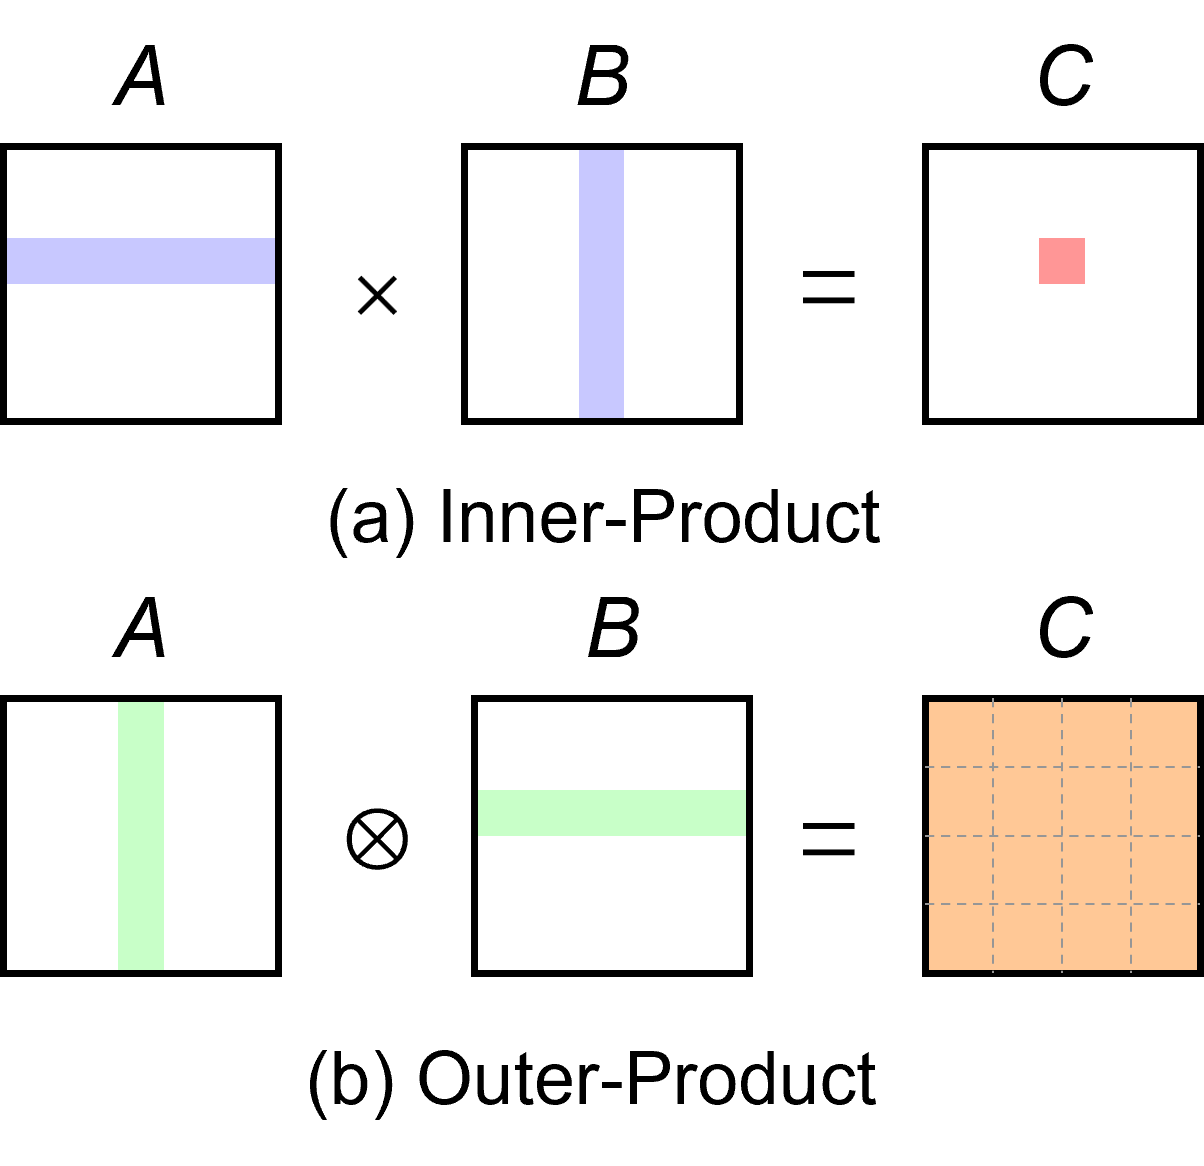
\includegraphics[width=0.95\linewidth]{figures/outerproduct.png}
    \caption{GEMM model of outer-product and inner-product.}
     \label{fig:outer_product_diagram}
\end{figure}

Arm processors have continuously expanded support for data-parallel and matrix-centric computation to satisfy increasing demand from HPC and AI workloads. Two architectural features, SVE and SME, are central to this trend. SVE provides a vector-length-agnostic SIMD model, while SME introduces a matrix-oriented outer-product execution model specialized for high-throughput accumulation (Figure~\ref{fig:outer_product_diagram}(b)). Understanding the execution semantics of these features is essential for the optimization of irregular GEMMs.

\textbf{SVE.} SVE~\cite{stephens2017arm} extends conventional SIMD through vector-length agnosticism. Instead of fixing vector width at compile time, SVE implementations expose vector lengths (VL) from 128 to 2048 bits in 128-bit increments. SVE also introduces predicate registers to control active lanes: each predicate element controls whether the corresponding lane is active, so inactive lanes are masked without control-flow divergence. This design handles loop tails and non-uniform trip counts efficiently without explicit scalar epilogues.

\textbf{SME.} SME builds on SVE and shifts the computational abstraction from lane-wise vectors to tile-wise accumulation. Architecturally, SME introduces the ZA matrix register file, a two-dimensional accumulator of $\mathit{VL} \times \mathit{VL}$ bytes that is logically partitioned into independent accumulator tiles. The number of tiles depends on element precision: element sizes of 1, 2, 4, 8, and 16 bytes correspond to 1, 2, 4, 8, and 16 tiles, respectively. Crucially, SME provides orthogonal access to ZA, allowing tiles to be read or written by either rows or columns without explicit data rearrangement. This eliminates software-level transposition and improves data reuse across tensor dimensions.

Computation in SME is driven by a hardware outer-product unit. Given a horizontal source vector $u$ and a vertical source vector $v$, the MOPA instruction computes their outer product and accumulates the result into a destination tile $D$:
$$
    D \leftarrow D + (u \otimes v).
$$
A single MOPA delivers $O(\mathit{VL}^2)$ operations and contributes a rank-1 update to the tile; repeated updates along the reduction dimension construct the final tile entirely in ZA. Because partial sums remain in ZA across many instructions, pressure on general vector registers is reduced and arithmetic intensity is much higher than what SVE alone can achieve.

For reduced-precision workloads, SME employs widening outer-product operations in which lower-precision inputs are multiplied and accumulated into wider-precision tiles. For example, FP16 inputs are accumulated into FP32 tiles via a two-way accumulation (pairs of adjacent FP16 elements are multiplied independently and summed into one FP32 element of the tile), preserving numerical robustness while increasing throughput compared with FP32 execution.

These benefits come with structural constraints. The efficiency of SME depends on matching problem dimensions with tile geometry, and the overhead of ZA data movement must be amortized by sufficient computation. Therefore, applying SME to irregular GEMMs---such as the tall-and-skinny shapes that dominate AlphaFold2---demands specialized optimization strategies to prevent severe performance degradation.

\subsection{The Architecture of 920F CPU}
% \subsection{The Architecture of 920F CPU}
% 920F CPU提供了OPA(Outer-Product Accumulator)以及配套的向量指令用于加速矩阵计算。920F使用一个array register来存储外积计算的结果，该array register可以被拆分为1个8-bits元素、2个16-bits元素、4个32-bits元素或8个64-bits元素的寄存器。对于每种数据类型，array register均含有VL(vector lenght) $\times$ VL个元素。OPA指令从将两个向量寄存器中的向量做外积，并累加到相应精度的array register上。920F 提供了int8、fp16、fp32、fp64的OPA指令。int8的OPA指令会将输入寄存器划分为4个向量，并在int32精度的array register上累加4组外积的结果。fp16的OPA指令会将输入寄存器划分为两个向量，并在fp32精度的array register上累加2组外积的结果。fp32与fp64则是直接在相应精度的array register上累加一组外积的结果。对于fp16(int8)的OPA指令，920F要求同一个输入寄存器内的向量是交织的，也即每个外积向量的元素索引之差为2(4)。

\begin{figure}[t]
    \centering
    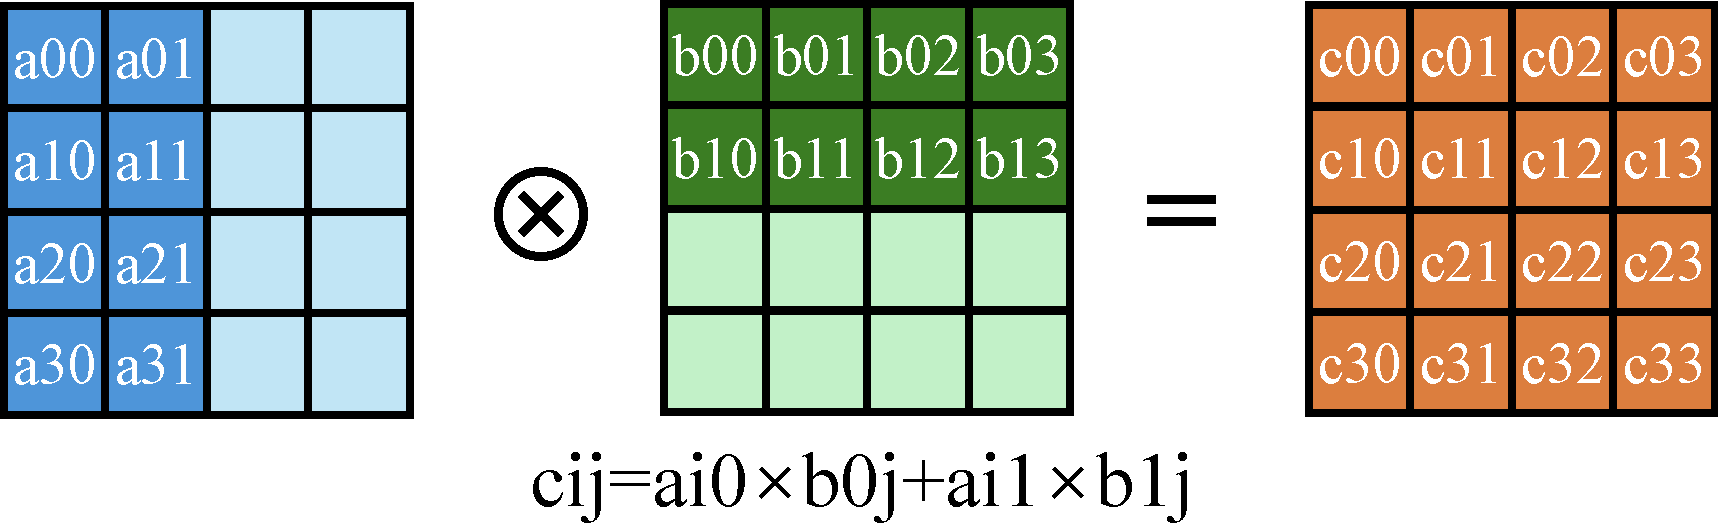
\includegraphics[width=0.8\linewidth]{figures/opa_2way.pdf}
    \caption{2-way OPA Instruction on 920F CPU.}
    \label{fig:opa}
\end{figure}

The 920F processor is a representative many-core ARM CPU that implements the SME extension described above. As a concrete instance of an outer-product-accumulator (OPA) architecture, it inherits the ZA matrix register file and MOPA-style execution semantics, while adding several platform-level characteristics that shape its performance profile.

\textbf{Many-core multi-NUMA organization.} A single 920F socket integrates more than 256 cores partitioned into 8 NUMA domains, with each core exposing its own per-core SME unit. The processor further provides high-bandwidth on-package memory and a dedicated memory movement unit for hardware-assisted bulk transfers. These features allow large activation tensors to remain on-package, which is particularly valuable for AlphaFold2 inference, but also introduce non-uniform access costs that must be managed by the software.

\textbf{Vector length and supported precisions.} The 920F implements a 512-bit vector length (VL = 512), so each ZA tile holds $64 \times 64$ FP16 elements or $16 \times 16$ FP32 elements after the standard precision-based partitioning. Native MOPA instructions are provided for FP32, FP16, and INT8 inputs. In this work, we focus on FP32 and FP16 computation modes.

\textbf{Two-way FP16 OPA.} As a concrete instantiation of the widening outer product, Fig.~\ref{fig:opa} illustrates the 2-way FP16 MOPA on 920F: each input vector register is interpreted as two interleaved sub-vectors of FP16 elements, and one instruction accumulates two FP16 outer products into a single FP32 destination tile. This interleaved operand layout is a hardware requirement: when the source data is stored row-major in memory, an explicit reinterpretation step is needed before the OPA can consume it. Section~\ref{sec:optimizations} discusses how we exploit ZA's orthogonal row/column access to perform this reinterpretation with minimal overhead.

% For quantized integer inference, the architecture leverages the reduced bit-width to perform a \textit{4-way outer product} ($K=4$), as illustrated in Fig.~\ref{fig:opa}.
% When operating on 8-bit integer (INT8) data, the source vectors are processed as groups of four consecutive elements. The hardware computes the outer product of a 4-element sub-vector from the row input and a 4-element sub-vector from the column input, accumulating the sum into a 32-bit integer (INT32) destination tile. By packing four 8-bit multiplications into a single accumulator update, this 4-way mechanism significantly increases the arithmetic intensity and allows for efficient utilization of the available memory bandwidth.



% \subsection{Mixed Precision Model Inference}
% Model quantization is a widely adopted technique in deep learning that reduces the precision of model parameters and intermediate activations to improve inference efficiency.~\cite{krishnamoorthi2018quantizing,polino2018model,jacob2018quantization} Instead of relying solely on high-precision floating-point formats such as FP32 or FP16, quantization typically converts data into lower-bit integer formats (e.g., INT8). This reduction not only decreases the memory footprint and data transfer volume but also allows hardware accelerators, including CPU matrix units, to perform more operations per cycle due to higher arithmetic density.

% % Quantization methods can be broadly categorized into two groups: post-training quantization (PTQ) and quantization-aware training (QAT). PTQ directly converts a pre-trained floating-point model into a lower-precision version, often requiring minimal additional computation. While PTQ is attractive for deployment, it may suffer from accuracy degradation, particularly for models with sensitive numerical operations. In contrast, QAT simulates quantization effects during training, enabling the model to adapt to low-precision arithmetic. This usually yields higher accuracy but requires additional training resources.

% Recent advances in quantization have demonstrated that many large-scale deep learning models in computer vision and natural language processing can be effectively quantized to INT8 with negligible accuracy loss. Furthermore, modern hardware platforms, including CPUs with specialized matrix units, provide native support for integer arithmetic, making quantization a natural fit for high-performance inference on general-purpose processors.

% However, applying quantization to AlphaFold2 introduces unique challenges. The model integrates heterogeneous computations, ranging from long-sequence attention to triangular updates and geometric transformations. These operations are not only memory-intensive but also highly sensitive to numerical precision. Small rounding errors during quantization can propagate and amplify through iterative refinement, potentially leading to distorted protein structures. Therefore, careful design of quantization strategies, including operator-level calibration, mixed-precision schemes, and error-compensation techniques, is essential to maintain prediction accuracy while benefiting from the efficiency of low-precision execution.

% \subsection{Statistics of AlphaFold2}
% \begin{figure*}[htbp]
%     \centering
%     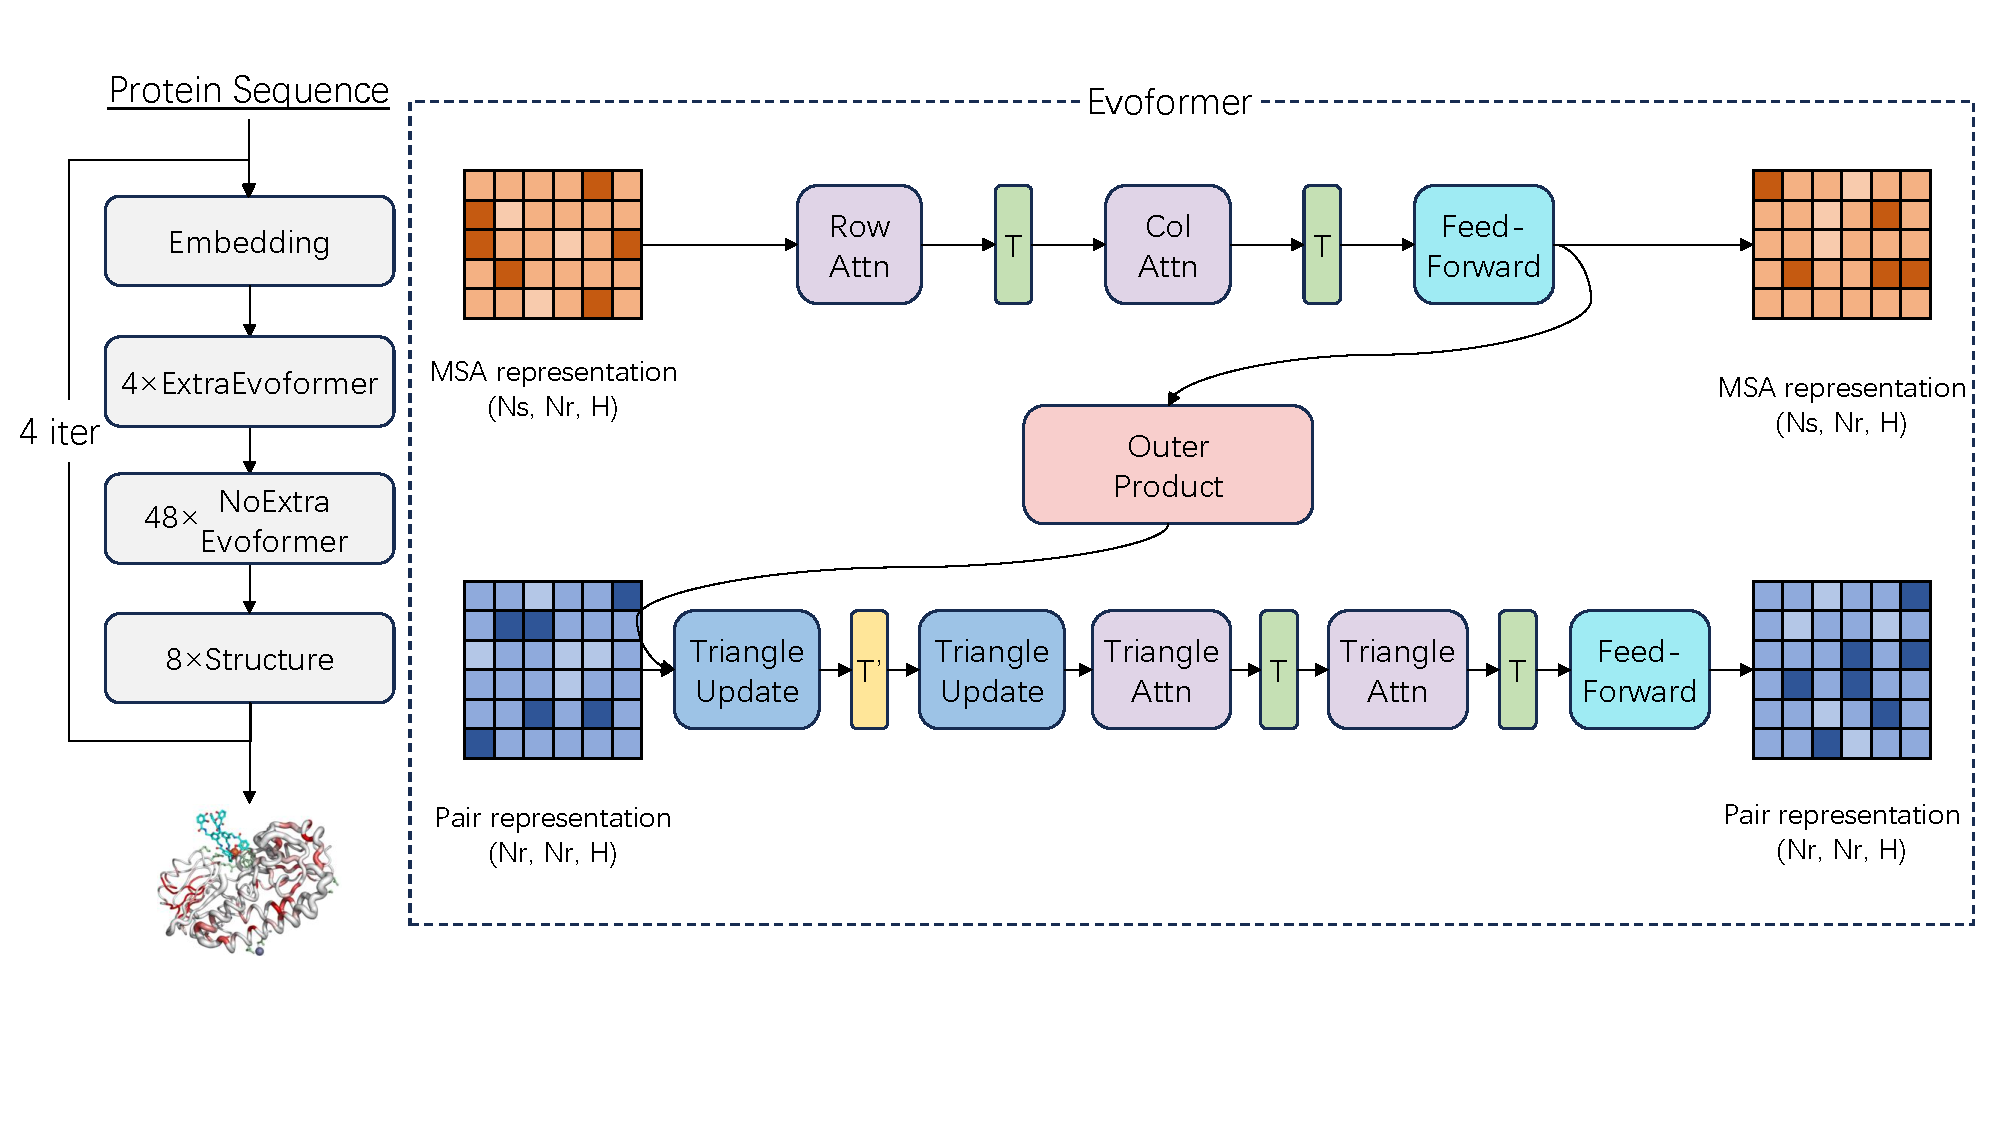
\includegraphics[width=\textwidth]{figures/AlphaFold.pdf}
%     \caption{AlphaFold2 Model Architecture}
%     \label{fig:af2model}
% \end{figure*}
% % AlphaFold2 adopts a highly modular architecture that integrates multiple neural network components to capture both local sequence features and long-range structural dependencies. The overall pipeline can be divided into three main stages: the Embedding Module, the Evoformer and the Structure Module.

% % The Evoformer is the central component that processes two key data representations: the multiple sequence alignment (MSA) features and pairwise residue features. It employs a combination of transformer blocks, attention mechanisms, and triangular multiplicative updates to model evolutionary relationships and inter-residue interactions. This stage is both compute- and memory-intensive, as it involves long-sequence attention operations and large tensor transformations.

% % The Structure Module takes the processed representations from the Evoformer and generates three-dimensional protein structures. It employs a recurrent geometry-based update procedure that iteratively refines atomic coordinates, ensuring that predicted conformations are physically consistent. This module involves numerous rigid-body transformations and specialized operations on rotation and translation groups, which differ from conventional deep learning layers.

% % Finally, AlphaFold2 relies on iterative refinement, where the Evoformer and Structure Module are applied multiple times to progressively improve prediction accuracy. This iterative nature further amplifies the computational demands of the model.

% AlphaFold2 has established a new paradigm in protein structure prediction by integrating deep learning with evolutionary and physical constraints. Given an amino acid sequence, AlphaFold2 predicts the three-dimensional atomic structure with an accuracy comparable to experimental methods such as X-ray crystallography~\cite{smyth2000x} and cryo-EM~\cite{bai2015cryo,earl2017cryo}. This breakthrough has had a profound impact on structural biology, drug discovery, and protein engineering, while also drawing significant attention from the computer systems community due to its computational complexity.

% As shown in Fig.~\ref{fig:af2model},
% AlphaFold2 consists of three major stages: input representation, Evoformer, and structure module.

% \textbf{Input representation.} The model first extracts features from the target protein sequence and its multiple sequence alignment (MSA). This process produces two key embeddings: a per-residue sequence embedding and a pairwise embedding that encodes residue-residue relationships.

% \textbf{Evoformer.} This stage is the computational core of AlphaFold2 and accounts for the majority of runtime and memory usage. The Evoformer is a deep stack of transformer-like blocks that iteratively refines both the MSA embedding and the pairwise embedding. Unlike standard NLP transformers, the hidden dimensions in AlphaFold2 are relatively small (typically 128 or 256), which means the memory footprint of model weights is modest. Instead, the memory bottleneck comes from activations, especially when processing long protein sequences, where both the MSA and pairwise representations can grow quadratically. Moreover, \textit{logits} in these modules exhibit cubic growth. Another distinctive feature is that the Evoformer alternates between intra-chain attention (within a single protein chain) and inter-chain attention (across multiple chains). These modules require frequent reshaping of data layouts. As a result, activation tensors are repeatedly transposed between different memory layouts, introducing additional communication overhead.

% \textbf{Structure module.} Using the refined representations, the structure module predicts 3D atomic coordinates. It relies on geometric reasoning over rotations and translations, converting pairwise features into structural constraints. Compared to the Evoformer, this stage is relatively lightweight in terms of computation, but essential for ensuring physically plausible predictions.

% From a systems perspective, AlphaFold2 exhibits several properties that distinguish it from typical deep learning workloads.

% \textbf{Activation-dominated memory footprint.} In contrast to large NLP models, AlphaFold2 has relatively small hidden dimensions, and thus, the memory contribution of model weights is minor. Instead, the dominant memory cost arises from activations, particularly for long sequences, where both MSA and pairwise representations scale with sequence length.

% % \textbf{Frequent communication due to tensor transpositions.} To enforce the physical plausibility of the protein structure, AlphaFold2 interleaves different types of attention and pairwise updates, many of which require switching tensor layouts. For example, intra-chain and inter-chain attention operate on different axes of the same tensor, leading to repeated transpose operations. These data movements create significant communication overhead, especially on architectures where cross-NUMA transfers are expensive.In Fig.~\ref{fig:af2model}, the transposition is denoted by \textit{T}, and \textit{T'} represents an equivalent transposition operation.

% \textbf{Dense linear algebra as the dominant computation.} Similar to other transformer-based models, AlphaFold2 is heavily dominated by matrix multiplications and other dense tensor operations, making it highly dependent on the efficiency of GEMM kernels and memory bandwidth.

% The activation-heavy memory usage, and dense linear algebra kernels together make AlphaFold2 both compute- and memory-intensive. In the next section, we present a detailed bottleneck analysis to quantify these challenges and identify the optimization opportunities for the 920F CPU.

% % From a systems perspective, AlphaFold2 presents several unique challenges compared to conventional vision or language models. First, its extensive use of attention across long MSAs leads to quadratic computational complexity with respect to sequence length. Second, the triangular updates and geometric transformations require substantial matrix multiplications interleaved with non-standard operations, making the workload heterogeneous and difficult to optimize. Third, the model's memory footprint is significant, as it maintains multiple high-dimensional feature tensors across iterations. These characteristics make AlphaFold2 particularly demanding for hardware platforms and motivate careful exploration of architectural accelerators such as matrix units on CPUs.

\section{AlphaFold2 Characteristics and Bottleneck Analysis}
\label{sec:analysis}

To identify the optimization opportunities and design constraints relevant to OPA-equipped CPUs, we first review the structure of AlphaFold2 and then quantify three system-level bottlenecks: dense GEMM computation, activation-dominated memory pressure, and frequent tensor-layout transformations. %The analysis proceeds top-down---from the overall model, to the workload breakdown across modules, to a detailed characterization of the dominant kernels.

\subsection{AlphaFold2 Model Overview}
\label{sec:analysis:model}

\begin{figure*}[t]
    \centering
    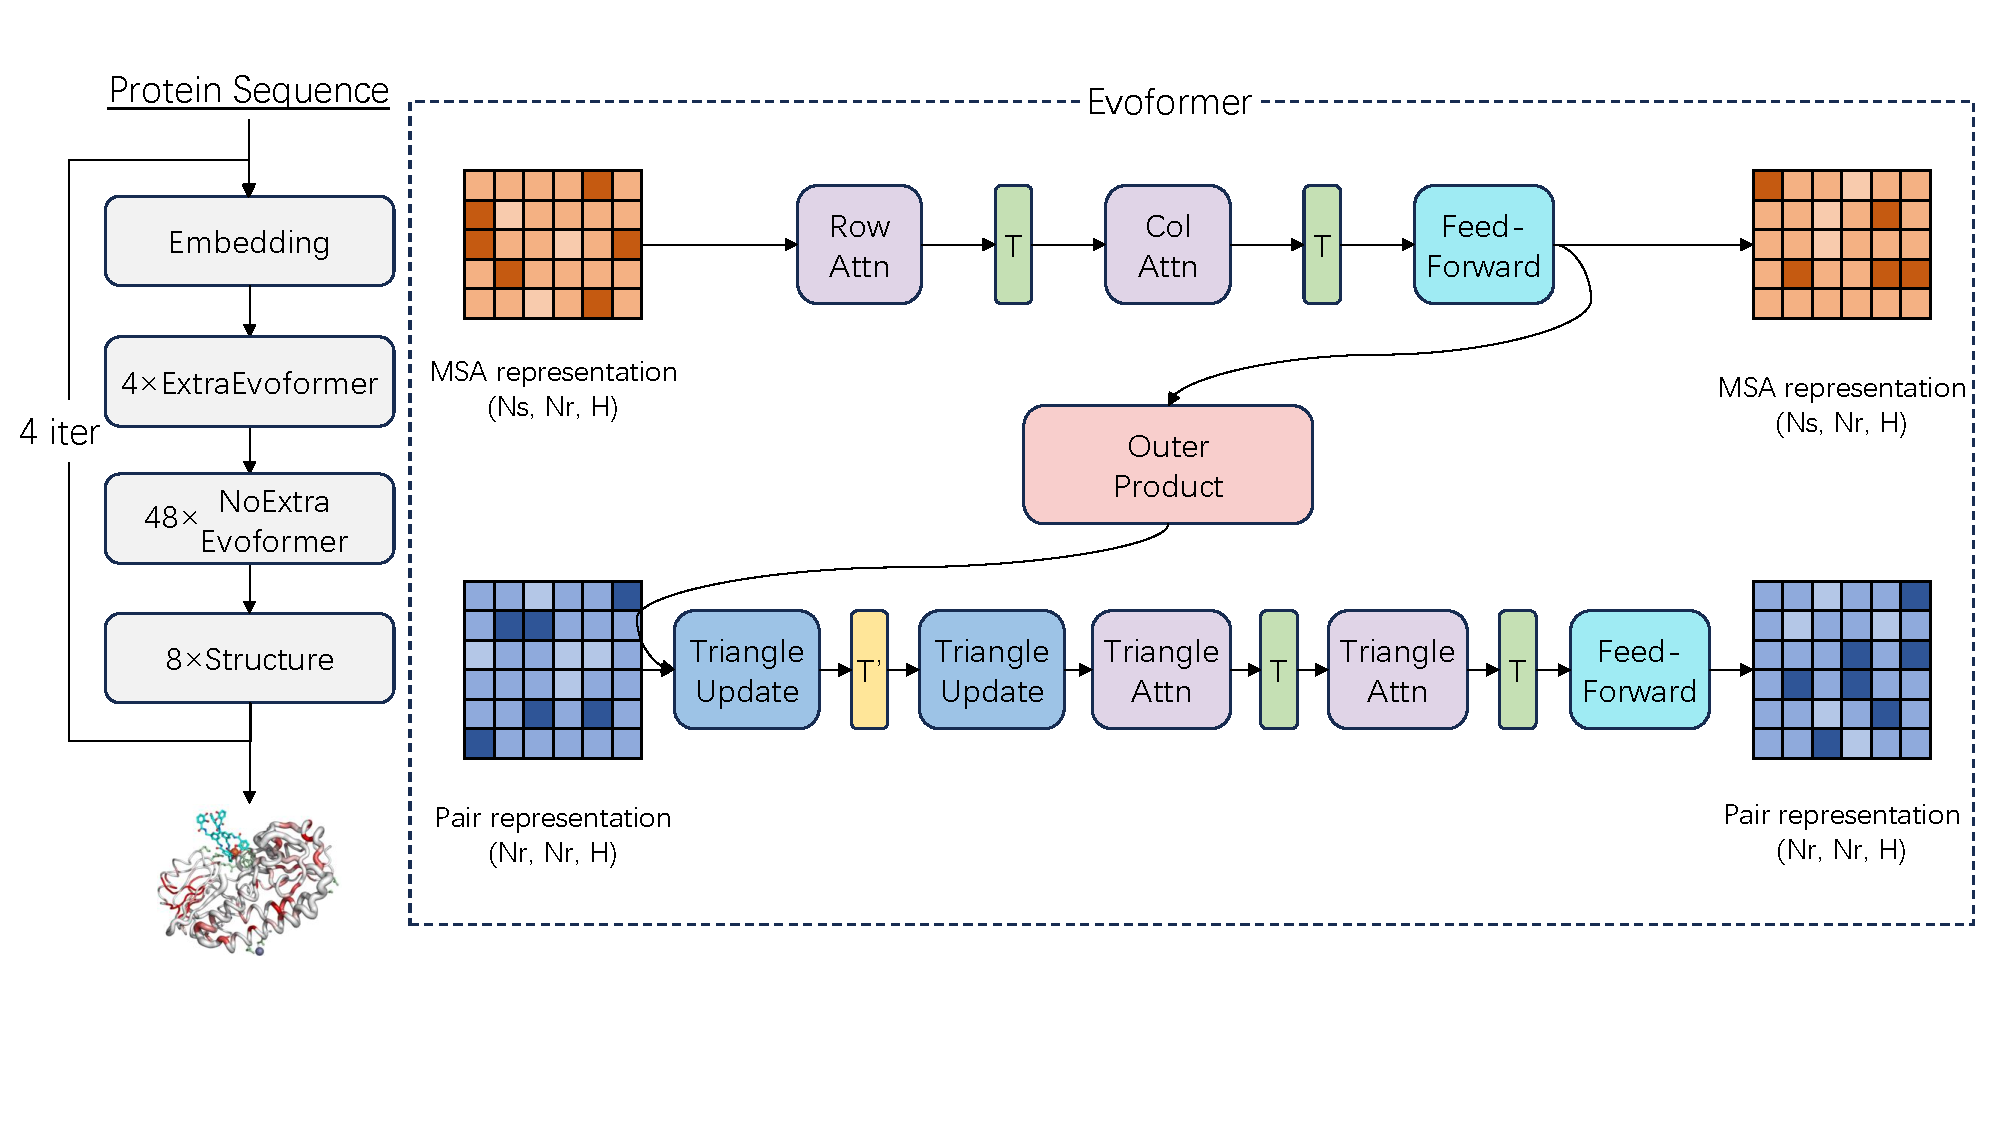
\includegraphics[width=0.95\textwidth]{figures/AlphaFold.pdf}
    \caption{AlphaFold2 model architecture. \textit{T} and \textit{T'} mark tensor transpositions between row-major and column-major layouts.}
    \label{fig:af2model}
\end{figure*}

AlphaFold2~\cite{jumper2021highly} predicts the three-dimensional structure of a protein from its amino acid sequence with near-experimental accuracy. As illustrated in Fig.~\ref{fig:af2model}, the model consists of three major components:

% \begin{itemize}
    \textbf{Input representation.} The model first searches for homologous sequences and assembles a multiple sequence alignment (MSA), then produces two embeddings: a per-residue MSA embedding of shape $N_s \times N_r \times c_m$ (where $N_s$ is the number of MSA rows and $N_r$ is the residue length) and a pairwise embedding of shape $N_r \times N_r \times c_z$. The hidden channel widths $c_m$ and $c_z$ are small, typically 128 or 256.

    \textbf{Evoformer.} A deep stack of transformer-like blocks iteratively refines the MSA and pairwise embeddings. Each block alternates row-wise and column-wise attention over the MSA, triangular multiplicative updates and triangular attention over the pairwise representation, and an outer-product-mean module that mixes information between the two streams. The blocks are repeated 48 times in the standard configuration.

    \textbf{Structure module.} Using the refined representations, the structure module recurrently predicts 3D atomic coordinates through invariant point attention and rigid-body updates, producing a physically plausible conformation.
% \end{itemize}

This architecture differs from typical NLP transformers in two important ways. First, the hidden dimensions ($c_m, c_z \in \{128, 256\}$) are an order of magnitude smaller than those of mainstream LLMs, which sharply reduces parameter count but, as we show below, also makes most GEMMs \textit{tall-and-skinny}. Second, the alternation between row-wise and column-wise operations on shared tensors mandates frequent layout transitions that have no counterpart in standard transformer stacks.

\subsection{Botttleneck Analysis}
% \subsection{Workload Breakdown}
% \label{sec:analysis:breakdown}

We profile AlphaFold2 inference at a representative residue length of $N_r = 1024$. The execution time decomposes as follows: the \textbf{Evoformer} accounts for approximately \textbf{75\%} of total runtime, the \textbf{structure module} for \textbf{13\%}, and the \textbf{embedding stage} for \textbf{11\%}. 

% First, the Evoformer is the unambiguous optimization target: any speedup on its constituent attention and triangular kernels translates almost directly into end-to-end gains. Second, the structure module and embedding stage are non-trivial in absolute terms; they are dominated by smaller, irregular operators whose latency cannot be amortized away by parallelism, so a CPU implementation must avoid leaving them serialized on a single thread. The remainder of this section therefore drills into the three system-level bottlenecks that the Evoformer in particular exposes.

% \subsection{Botttleneck}
\subsubsection{Dense GEMM with Tall-and-Skinny Shapes}
\label{sec:analysis:shape_dist}

\begin{figure}[t]
    \centering
    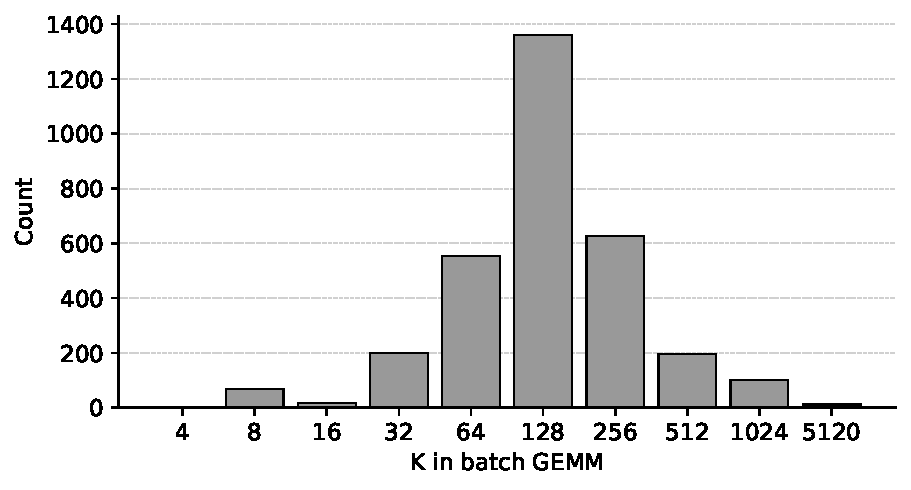
\includegraphics[width=\linewidth]{figures/shape_dist.pdf}
    \caption{Distribution of batched GEMM K dimensions over one Evoformer iteration of AlphaFold2 inference.}
    \label{fig:k_dist}
\end{figure}

Like other models based on transformers, the Evoformer is dominated by dense matrix multiplications: linear projections in attention, the Q/K/V/output GEMMs, the gated MLP that follows each attention block, and the bilinear updates inside the triangular multiplicative module. On an OPA architecture, the performance of these GEMMs is governed primarily by the reduction dimension $K$, for two reasons.

\textbf{Why $K$ matters on OPA.} Each MOPA instruction performs a rank-1 update directly into a ZA tile, so a complete GEMM tile is constructed by issuing $K$ MOPAs along the reduction axis and then \textit{draining} the tile back to memory. The drain step, which is absent from conventional FMA-based CPU GEMMs, is a fixed cost per output tile. As a result, the GEMM execution can be modelled as a four-stage pipeline: operand load, MOPA accumulation, tile drain, and writeback. The throughput is determined by how well MOPAs amortize the drain and writeback. When $K$ is large, the MOPA stage dominates and the kernel approaches peak compute throughput; when $K$ is small, drain and writeback occupy a comparable or larger fraction of the issue slots, and the kernel becomes memory- and instruction-bandwidth bound.

\textbf{The shape distribution in AlphaFold2.} Fig.~\ref{fig:k_dist} reports the distribution of $K$ across all batched GEMMs in a single Evoformer iteration. GEMMs with $K \le 256$ account for the dominant share of operator instances. This pattern is a direct consequence of AlphaFold2's small channel widths ($c_m, c_z \in \{128, 256\}$) and of attention being executed as batched per-head GEMMs with per-head dimension $c/N_{\text{heads}} = 32$ or $64$. The same hidden dimension that keeps the model parameter-efficient turns out to make every projection GEMM tall-and-skinny.

A small $K$ does not imply a small workload. These tall-and-skinny GEMMs typically come paired with large $M$, $N$, or batch dimensions. So their total FLOP count is comparable to, and often exceeds, that of the few large-$K$ GEMMs in the model. The optimization problem is how to make the OPA pipeline efficient at small $K$, which we address in Section~\ref{sec:optimizations}.

\subsubsection{Activation-Dominated Memory Pressure}
\label{sec:analysis:memory}

A second distinguishing property of AlphaFold2 is that its memory footprint is dominated by \textit{activations} rather than weights. With $c_m, c_z \le 256$, the parameter set is modest in size, but the intermediate tensors scale super-linearly in the input length:
\begin{itemize}
    \item the MSA representation grows as $O(N_s N_r c_m)$,
    \item the pairwise representation grows as $O(N_r^2 c_z)$,
    \item the attention logits ($Q K^\top$) grow as $O(N_s N_r^2)$ for MSA attention or $O(N_r^3)$ for triangular attention.
\end{itemize}

The cubic term is the binding constraint at long sequences. For example, when $N_r$ approaches a few thousand residues, a single triangular-attention logits tensor can consume tens of GiB, exceeding the on-package memory of many accelerators. The standard remedy is to chunk the attention computation along the batch or head dimension and stream tiles through fast memory.~\cite{zhao2024autochunk} Chunking trims peak memory linearly in the chunk size but it shrinks the per-tile workload exposed to parallel hardware.

% The implication for the 920F platform is two-sided. On one hand, the on-package memory is large enough that chunk sizes can remain comparatively generous, preserving more parallelism than a memory-constrained GPU could afford. On the other, once $N_r$ grows past the on-package capacity, the working set spills to off-chip memory and locality degrades---an effect that we observe directly in the long-sequence regime of our evaluation (Section~\ref{sec:end_to_end}).

\subsubsection{Frequent Tensor Layout Transformations}
\label{sec:analysis:comm}

The Evoformer is unusual among transformer architectures in that successive operators within the same block act along \textit{different} tensor axes. MSA row-wise attention contracts along the residue axis, MSA column-wise attention contracts along the sequence axis, and the triangular multiplicative module updates the pairwise tensor first along one residue axis and then along the other. To express each of these operators as a contiguous, vectorizable contraction, the implementation must transpose the underlying tensor between row-major and column-major layouts, which are marked $T$ and $T'$ in Fig.~\ref{fig:af2model}.

Each transposition has two costs on a many-core CPU. The first is data movement: transposing an MSA or pairwise activation touches every element of the tensor, and on a multi-NUMA node these elements are partitioned across local memories, so the transpose generates remote traffic that is bottlenecked by the inter-NUMA interconnect rather than by local DRAM bandwidth. The second is synchronization: when the workload is parallelized along the sequence or residue axis, every transpose acts as a barrier between the producers (which write along one axis) and the consumers (which read along the orthogonal axis). Both costs grow with activation size and therefore with sequence length.
Each block issues several layout transitions, and with 48 blocks per inference the cumulative cost becomes a non-trivial fraction of end-to-end runtime on long inputs. %The implication for our design is that minimizing the \textit{number} of transitions, and absorbing the residual ones into operator boundaries, is at least as important as accelerating the GEMMs themselves.

% \subsection{Summary}
% \label{sec:analysis:summary}

% The three bottlenecks above motivate a corresponding set of design decisions:
% \begin{enumerate}
%     \item Tall-and-skinny GEMMs require an OPA-aware kernel that aggressively amortizes the drain and writeback stages---addressed in Section~\ref{sec:optimizations} via a $K$-unblocked kernel and a tensor layout that matches the OPA operand format.
%     \item Activation-dominated memory pressure favours platforms with large on-package memory and rewards careful precision selection, which our FP16 mixed-precision strategy exploits.
%     \item Layout transpositions and NUMA traffic call for shared-memory communication primitives and a length-aware parallelism strategy that confines short sequences to a single NUMA node.
% \end{enumerate}

% The remainder of the paper develops these mechanisms in turn.

% \input{preliminaries}
%\input{challenges}
\section{Methodology}
\subsection{Matrix Format Design}
% 对于int8与fp16精度的OPA指令，72F要求输入寄存器内的向量是交织的。如果在寄存器中将标准row-major的矩阵进行重排，需要插入大量的寄存器操作指令。在72F上，单条数据排布指令与单条OPA指令的延迟类似，且难以与OPA指令重叠。这些指令会极大程度上拖慢OPA指令的执行速度。为了避免这种情况，我们设计了一个新的矩阵数据格式，称为Interleaved Matrix Format (IMF)。IMF将矩阵的行元素交织存储，使得每个向量寄存器中的元素可以直接用于OPA指令，而无需额外的重排操作。通过将GEMM的kernel设计为可以接收与输出IMF格式，我们可以避免大量的数据排布开销，而仅仅需要在算子入口处进行一次数据格式转换。
\subsection{Kernel Design}
\section{Evaluation}
\subsection{Experimental Setup}
% 我们的实验一共在两个Cluster上进行。在Cluster A上，我们在72F CPU上评估了MFold的性能。同时，我们将Cluster B上运行的FastFold{\color{red}~\cite{}}作为我们的基线。每个Cluster的具体配置如表~\ref{tab:cluster}所示。
We evaluate our optimizations on two distinct computing environments. The primary environment is a CPU cluster that serves as the optimization target of this work. The cluster is equipped with two 72F processors, each consisting of 8 NUMA nodes. Unless otherwise stated, all reported CPU results are obtained on a single 72F processor, which allows us to highlight the effectiveness of our optimizations without the influence of inter-socket communication overhead. This platform provides not only high computational throughput but also specialized matrix computation units, which we exploit to accelerate AlphaFold2 inference.

For comparison, we benchmark against FastFold, a state-of-the-art GPU-accelerated implementation of AlphaFold2. FastFold experiments are conducted on a server equipped with two Intel(R) Xeon(R) Gold 6336Y processors and a single NVIDIA A100 GPU. This configuration represents the mainstream deployment setting for AlphaFold2 inference on GPUs and provides a strong baseline to evaluate the competitiveness of our CPU-based optimizations.

Our evaluation dataset consists primarily of protein sequences from CASP14, which is widely adopted as a standard benchmark for protein structure prediction. Using CASP14 ensures that our results are comparable with prior studies and faithfully reflect AlphaFold2's predictive capability under realistic inference workloads.

It is worth noting that our optimized implementation achieves inference performance on a single 72F processor that matches or even surpasses that of an A100 GPU running FastFold, highlighting the potential of CPU-based acceleration with matrix units and quantization techniques.
\begin{table}
% Table generated by Excel2LaTeX from sheet 'Sheet1'
\begin{tabular}{|c|c|c|}
    \hline
    Cluster & A   & B \bigstrut\\
    \hline
    \hline
    CPU & 72F & Intel(R) Xeon(R) Gold 6336Y \bigstrut\\
    \hline
    Core & more than 256 & 24 \bigstrut\\
    \hline
    Memory &     & 512GB DDR4 \bigstrut\\
    \hline
    GPU & -   & A100 \bigstrut\\
    \hline
    System &     & Ubuntu 22.04 Linux 5.15.0 \bigstrut\\
    \hline
    \end{tabular}%
    
\caption{Cluster Configuration}
\label{tab:cluster}%
\end{table}

\subsection{End to End Performance Comparison}
% 我们从CASP14中选择了从长度32到2180的不同的数据进行了测试。对比结果如图~\ref{fig:endtoend}所示。

\subsection{Attention Kernel Performance}
% 由于我们的MFold实现与FastFold并未共享同一pipeline，为了更加充分的展示加速的效果，我们对比了MFold的fp16、int8精度以及Fastfold的Attention模块的性能。我们使用了从32~4096的不同长度的序列进行测试。对比结果如图~\ref{fig:attention}所示。
%\input{casestudy}
\section{Related Work}
\label{sec:relatedwork}
% \subsection{AlphaFold2 implementations}. 
% A large body of work targets training and inference efficiency on GPUs. 
% OpenFold~\cite{ahdritz2024openfold} reimplements AlphaFold2 with a focus on trainability and memory efficiency, matching AlphaFold2 accuracy while improving training throughput; industry reports describe additional engineering that shortens large-scale training on multi-GPU clusters. 
% FastFold~\cite{cheng2024fastfold} introduces Dynamic Axial Parallelism, Duality Async Operations, and AutoChunk, reporting reductions in training time and substantial speedups for long-sequence inference; later studies further systematize GPU-cluster optimizations for AlphaFold-style workloads. 
% Uni-Fold provides an open-source platform for AlphaFold with engineering improvements to training and inference pipelines. 
% 尽管这些工作在GPU上取得了一定的加速效果，但它们并未针对CPU进行优化。

% MSA and data-pipeline acceleration. Since MSA dominates wall-clock time in many deployments, the ColabFold stack replaces JackHMMER/HHblits with MMseqs2, yielding large end-to-end speedups; subsequent GPU implementations of MMseqs2 report further gains and integrate with ColabFold. These works primarily optimize the search pipeline rather than the AlphaFold2 neural kernels themselves. 

% Operator/memory specialization and long-sequence inference. Beyond parallelism, recent efforts study memory-aware chunking and kernel choices inside the Evoformer to support longer sequences with lower memory, often building on FastFold's ideas. 

% Scope relative to this work. Existing efforts overwhelmingly target GPU execution and/or MSA acceleration. To our knowledge, there is no prior systematic study that (i) optimizes AlphaFold2 inference on many-core CPUs with matrix units, and (ii) combines INT8 quantization with OPA-style kernels and NUMA-aware execution to deliver competitive end-to-end latency. Our work fills this gap by focusing on CPU-resident kernels, layout transformations, and quantization strategies tailored to AlphaFold2’s heterogeneous computation. (We base this claim on the surveys and implementations cited above.)
% Recent years have seen a surge in research focused on optimizing the training and inference efficiency of AlphaFold2, a landmark model in protein structure prediction.[1] The majority of these efforts have centered on leveraging the parallel processing capabilities of GPUs and implementing the model more efficiently.
\subsection{Optimizations for AlphaFold2}
% Since the release of AlphaFold2, a significant body of work has been dedicated to optimizing its computational pipeline for both training and inference. The majority of these efforts have focused on leveraging massively parallel hardware, primarily GPUs. For instance, OpenFold~\cite{ahdritz2024openfold} presented a faithful reimplementation of AlphaFold2 that matches the original's accuracy while significantly improving training throughput and memory efficiency, enabling training on fewer GPUs. FastFold~\cite{cheng2024fastfold} introduced several algorithmic innovations, including Dynamic Axial Parallelism and Duality Async Operations, to report substantial reductions in both training time and end-to-end inference latency, especially for long protein sequences. Similarly, Uni-Fold~\cite{li2022uni} provided an open-source PyTorch implementation with engineering enhancements that accelerated the training process compared to the official JAX-based code. ParaFold~\cite{zhong2022parafold} is an optimized system for AlphaFold inference on heterogeneous platforms, focusing on optimizing the data processing workflow. 

% While GPU-centric optimizations are prevalent, some research has explored accelerating AlphaFold2 on CPUs. The APACE framework~\cite{park2024apace} was designed to speed up AlphaFold2 in HPC environments through CPU and GPU co-optimization, parallelizing the computationally demanding MSA and template search stages. Separately, Intel has demonstrated significant inference speedups on its Xeon CPUs by leveraging hardware features like AMX with bfloat16 precision.

% In contrast to these previous efforts, our work presents the first optimization of AlphaFold2 on a many-core CPU architecture (the 72F). While prior CPU-based work focused on general parallelization or utilized bfloat16 precision on conventional CPUs, our approach is the first to exploit the dedicated matrix computation units inherent to each core of the 72F, enabling efficient low-precision inference.

Efforts to optimize AlphaFold2 have largely focused on GPUs~\cite{ahdritz2024openfold,zhu2024scalefold,cheng2024fastfold,zhong2022parafold,li2022uni,villegas2023manyfold}. OpenFold~\cite{ahdritz2024openfold} presented a faithful reimplementation of AlphaFold2 that matches the original's accuracy while significantly improving training throughput and memory efficiency, enabling training on fewer GPUs. FastFold~\cite{cheng2024fastfold} introduced several algorithmic innovations, including Dynamic Axial Parallelism and Duality Async Operations, to report substantial reductions in both training time and end-to-end inference latency, especially for long protein sequences. Similarly, Uni-Fold~\cite{li2022uni} provided an open-source PyTorch implementation with engineering enhancements that accelerated the training process compared to the official JAX-based code. ParaFold~\cite{zhong2022parafold} is an optimized system for AlphaFold inference on heterogeneous platforms, focusing on optimizing the data processing workflow. While most work is GPU-centric, some has targeted CPUs. For instance, APACE~\cite{park2024apace} used CPU and GPU co-optimization in HPC environments. Open-Omics-AlphaFold~\cite{openomicsalphafold} accelerates AlphaFold through AMX on Intel CPUs. In contrast, our work focuses on exploiting the dedicated outer product units of a many-core CPU architecture (72F) for low-precision inference, a departure from prior CPU optimizations focused on general parallelism.
% \subsection{Model Mixed-Precision and Quantization}

% Model quantization is a recognized technique for reducing computational and memory costs by using lower-precision numerical formats for model weights and activations.[19] While general-purpose INT8 quantization for large neural networks is a mature field, its application to complex models in protein structure prediction remains limited.[20][21] Some studies have investigated post-training quantization (PTQ) for protein language models like ESMFold.[22] However, these efforts have highlighted challenges, noting that standard 8-bit quantization methods can lead to a significant drop in prediction accuracy for these specialized models.[22]
% Model quantization is a well-established technique for reducing the memory footprint and computational cost of deep learning models by using lower-precision numerical formats, such as 8-bit integers (INT8). Early methods often combined quantization with knowledge distillation to help the smaller, quantized model recover the accuracy of the larger, full-precision model~\cite{polino2018model}. However, the advent of the Transformer architecture, which is a core component of AlphaFold2's Evoformer blocks, introduced new challenges.
% The primary difficulty in quantizing Transformers lies in the high dynamic range of their activation values. Large-magnitude outliers in activations can severely degrade the accuracy of standard quantization schemes. To address this, Dettmers et al. proposed GPT3.INT8()~\cite{dettmers2022gpt3}, a mixed-precision approach that performs matrix multiplication in INT8 for most features but uses FP16 for the outlier features, effectively preserving model performance. An alternative solution, SmoothQuant~\cite{xiao2023smoothquant}, introduced an offline, mathematically equivalent transformation that smooths activation outliers by migrating the quantization difficulty from activations to weights, enabling accurate and efficient INT8 quantization for both. More recently, work has also focused on specific Transformer components, with methods like SageAttention~\cite{zhang2024sageattention} being developed to enable accurate 8-bit attention calculations specifically.
% Despite these significant advances, which have been predominantly validated on large language models (LLMs), their application to scientific computing models like AlphaFold2 remains an open challenge. To our knowledge, no prior work has successfully navigated these challenges to implement and validate a full INT8 quantization scheme for the entire AlphaFold2 model. Our work is the first to do so, developing a methodology to apply both FP16 and, more importantly, INT8 precision to the AlphaFold2 inference pipeline while maintaining high accuracy. 
% Model quantization reduces compute and memory costs using low-precision formats like 8-bit integers (INT8). Significant progress has been made for large language models (LLMs), with techniques like the mixed-precision approach in GPT3.INT8() of Dettmers et al.~\cite{dettmers2022gpt3}. An alternative solution, SmoothQuant~\cite{xiao2023smoothquant}, introduced an offline, mathematically equivalent transformation that smooths activation outliers by migrating the quantization difficulty from activations to weights, enabling accurate and efficient INT8 quantization for both. More recently, work has also focused on specific Transformer components, with methods like SageAttention~\cite{zhang2024sageattention} being developed to enable accurate 8-bit attention calculations specifically.

% A central challenge in applying these methods to AlphaFold2 is the memory consumption, which is overwhelmingly dominated by activations rather than weights. The numerical distribution of these activations is highly sensitive to the input protein sequence, which makes traditional static quantization extremely difficult.
% The logical alternative is dynamic quantization, where scaling factors are computed on-the-fly for each input tensor. However, the computational overhead of calculating these factors in real-time can easily negate the performance gains from int8 matrix multiplications, posing a significant implementation challenge for achieving actual speedups.

\subsection{Other Protein Models}
Beyond AlphaFold2, other high-accuracy models have significantly advanced the field.~\cite{xu2019distance,zhou2022tasser} RoseTTAFold~\cite{baek2021accurate}, developed concurrently, achieved comparable performance using a similar deep learning architecture. Both models build upon foundational concepts from the MSA Transformer~\cite{rao2021msa}, which first demonstrated the power of attention mechanisms for processing co-evolutionary data. A different paradigm was introduced by ESMFold~\cite{lin2022language}, which leverages a large protein language model to predict structures from a single sequence, dramatically accelerating inference by bypassing the costly MSA search.

Critically, a common architectural motif unites these leading models: the extensive use of \textit{Evoformers} for iterative information refinement. This shared foundation means that the optimization techniques developed in our work are broadly applicable. Our methods for acceleration on dedicated CPU matrix units are not limited to AlphaFold2 but can be adapted to other Evoformer-based models like RoseTTAFold and ESMFold, making the proposed techniques attractive for other protein structure prediction models on CPU-centric systems.
Therefore, MatrixFold contributes to a more scalable and practical ecosystem for biological science.
\section{Conclusion}
% This work revisits CPU-based acceleration of AlphaFold2 in light of recent architectural innovations in many-core processors. By leveraging the 72F’s matrix units and integrating quantization into the computation pipeline, MatrixFold achieves competitive performance with GPU implementations and, crucially, outperforms the A800 GPU on long-sequence inference where memory capacity becomes a limiting factor for GPUs. Our NUMA-aware communication and adaptive parallelism strategies ensure efficient scaling across diverse sequence lengths. Experimental results on CASP14 confirm that both FP16 and INT8 quantization maintain reliable accuracy while substantially reducing inference latency. Beyond AlphaFold2, the techniques proposed in MatrixFold are applicable to other Evoformer-based models such as RoseTTAFold and ESMFold, highlighting the broader impact of CPU-based quantized inference. This study demonstrates that CPUs with matrix extensions are not only viable but can exceed top-tier GPUs in large-scale protein structure prediction workloads.
In this paper we demonstrate that through systematic hardware-software co-design, the computationally intensive AlphaFold2 model can be efficiently accelerated on modern many-core CPUs equipped with dedicated matrix units. Our proposed framework, MatrixFold, significantly boosts inference performance by integrating specialized GEMM kernels, an optimized multi-NUMA communication strategy, an adaptive parallelism mechanism, and the first application of INT8 quantization for AlphaFold2 on a CPU platform.
Beyond AlphaFold2, the techniques proposed in MatrixFold are applicable to other Evoformer-based models such as RoseTTAFold and ESMFold, highlighting the broader impact of CPU-based quantized inference. 

Our evaluation reveals that MatrixFold is not only highly competitive in performance but also maintains prediction accuracy comparable to the FP32 baseline. Critically, for long protein sequences, its performance surpasses that of state-of-the-art GPU solutions on NVIDIA A800.
This study demonstrates that CPUs with matrix extensions are not only viable but can exceed top-tier GPUs in large-scale protein structure prediction workloads.


%% Bibliography
\bibliography{ref}

\end{document}
